\PID 
Континуални сигнал $x(t) = \ee^{-at} \uu(t)$, где је $a > 0$ позната константа, 
доводи се на филтар пропусник ниских учестаности као на слици. 
Амплитудска фреквенцијска карактеристика филтра је 
$|H(\jj\upomega)| = \begin{cases}
    1 ,& |\upomega| \leq \upomega_0 \\
    0 ,& \text{иначе}
\end{cases}$, где је $\upomega > 0$ гранична учестаност тог филтра.
Одредити израз за енергију сигнала $y(t)$ на излазу филтра, $W_y$. Добијени резултат
графички представити.

\RESENJE
Одзив система у временском домену одређује се конволуцијом као $y(t) = x(t) \ast h(t)$, применом својства Фуријеове трансформације о конволуцији из додатка 
\ref{a:svojstva} има се veza $Y(\jj\upomega) = X(\jj\upomega) \cdot H(\jj\upomega)$, где су 
$Y(\jj\upomega) = \FT{y(t)}$, $X(\jj\upomega) = \FT{x(t)}$, и $H(\jj\upomega) = \FT{h(t)}$. Фуријеова трансформација импулсног 
одзива филтра стога се назива и \textit{функцијом преноса} филтра.

Амплитудски спектар представља модул Фуријеове трансформације, а амплитудска фреквенцијска карактеристика модул функције преноса па је 
$|Y(\jj\upomega)| = |X(\jj\upomega)| \cdot |H(\jj\upomega)|$. На основу Парсевалове теореме за Фуријеову трансформацију континуалног 
сигнала \eqref{s:ctft:parseval} је 
\begin{equation}
    W_y = \int_{-\infty}^{\infty} |y^2(t)|\,\de t = 
    \dfrac{1}{2\uppi}\int_{-\infty}^{\infty} |Y(\jj\upomega)|^2 \de \upomega. \label{eq:\ID.1}
\end{equation}
%
\begin{figure}[b!]
    \centering
    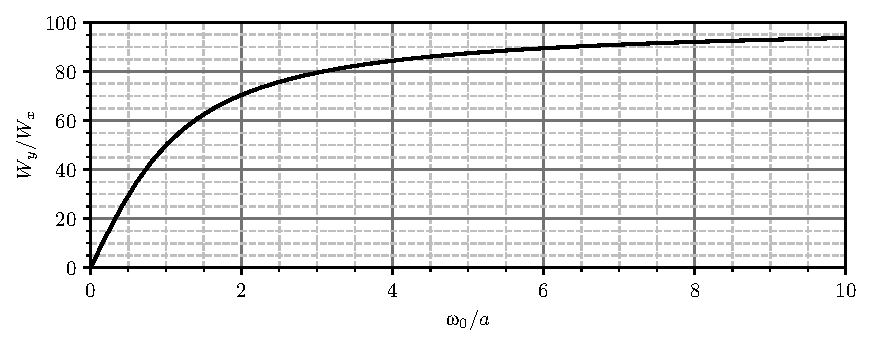
\includegraphics{fig/energija_wy.pdf}
    \caption{Уз решење задатка.}
    \label{fig:\ID.2}
\end{figure}
%
На основу датог израза има смисла величину $|Y(\jj\upomega)|^2$ назвати и \textit{спектралном густином енергије} 
датог сигнала. На основу табличне трансформације \reft{T:ctft:exp} је 
$X(\jj\omega) = \dfrac{1}{a + \jj\upomega}$, па се за спектралну густину снаге излазног сигнала може писати\footnote{
    Користе се идентитети  $|z/v| = |z|/|v|$, ($z,v\in\mathbb C$) и $|a +\jj b|^2 =  a^2 + b^2$, ($a,b \in \mathbb R$).
}
\begin{equation}
    |Y(\jj\upomega)|^2 = |X(\jj\upomega)|^2 \cdot |H(\jj\upomega)|^2 
    = \dfrac{1}{a^2 + \upomega^2} \cdot \begin{cases}
        1 ,& \upomega < \upomega_0 \\
        0 ,& \upomega > \upomega_0
    \end{cases}
\end{equation} 
Тражени резултат добија се заменом у \ref{eq:\ID.1} и применом табличног интеграла\footnote{
    Таблични интеграл који се користи је 
    $
    \int \dfrac{1}{1 + x^2} \, \de x = \arctan(x)
    $.
}
\begin{equation}
    W_y = 
    \dfrac{1}{2\uppi} \int_{-\upomega_0}^{\upomega_0} \dfrac{1}{a^2 + \upomega^2}  \de \upomega
    = \dfrac{1}{\uppi a} \int_{\upomega = 0}^{\upomega_0} \dfrac{1}{1 + (\upomega/a)^2}  \de (\upomega/a)
    = \dfrac{1}{\uppi a} \arctan\left( \dfrac{\upomega_0}{a} \right) \label{eq:\ID.2}
\end{equation}
Приметимо да је у случају $\upomega_0 \to \infty$ онда $H(\jj\upomega) = 1$, односно, $Y(\jj\upomega) = X(\jj\upomega)$. Природно, 
бесконачно широк НФ филтар пропушта све учестаности, па је погодно резултат \eqref{eq:\ID.2} изразити у облику 
\begin{equation}
    W_y = \underbrace{\dfrac{1}{2a}}_{W_x} \dfrac{2}{\uppi} \arctan\left(\dfrac{\upomega_0}{a}\right).
\end{equation}
Добијени резултат се онда смислено може графички представити како је приказано на слици \ref{fig:\ID.2}.
